\documentclass[aspectratio=169,11pt,hyperref={colorlinks=true}]{beamer}
\usetheme{boxes}
\setbeamertemplate{navigation symbols}{}
\definecolor{ibm}{RGB}{70,107,176}
\setbeamercolor{titlelike}{fg=ibm}
\setbeamercolor{structure}{fg=ibm}
\hypersetup{colorlinks,urlcolor=ibm}
\setbeamertemplate{footline}[frame number]
% Inserting graphics
\usepackage{graphicx}
% Side-by-side figures, etc
\usepackage{subfigure}
% Code snippits
\usepackage{listings}

\usepackage{lmodern}
% Color stuff
\usepackage{color}
\usepackage{amsmath}
\usepackage{amssymb}
\usepackage{empheq}
\usepackage[braket, qm]{qcircuit}
\usepackage{tikz}
\usepackage{gensymb}
\newcommand\RBox[1]{%
  \tikz\node[draw,rounded corners,align=center,] {#1};%
}
\usepackage{hyperref}
%\usecolortheme{buzz}
%\usecolortheme{wolverine}
%\usetheme{Boadilla}
\usepackage[T1]{fontenc}

\definecolor{mygreen}{rgb}{0,0.6,0}
\definecolor{mygray}{rgb}{0.5,0.5,0.5}
\definecolor{mymauve}{rgb}{0.58,0,0.82}

\lstset{%
  backgroundcolor=\color{white},   % choose the background color; you must add \usepackage{color} or \usepackage{xcolor}
  breakatwhitespace=false,         % sets if automatic breaks should only happen at whitespace
  breaklines=true,                 % sets automatic line breaking
  captionpos=b,                    % sets the caption-position to bottom
  commentstyle=\color{ibm},  % comment style
  extendedchars=true,              % lets you use non-ASCII characters; for 8-bits encodings only, does not work with UTF-8
  keepspaces=true,                 % keeps spaces in text, useful for keeping indentation of code (possibly needs columns=flexible)
  keywordstyle=\color{blue},       % keyword style
%  otherkeywords={*,...},           % if you want to add more keywords to the set
  numbersep=5pt,                   % how far the line-numbers are from the code
  numberstyle=\tiny\color{mygray}, % the style that is used for the line-numbers
  rulecolor=\color{black},         % if not set, the frame-color may be changed on line-breaks within not-black text (e.g. comments (green here))
  showspaces=false,                % show spaces everywhere adding particular underscores; it overrides 'showstringspaces'
  showstringspaces=false,          % underline spaces within strings only
  showtabs=false,                  % show tabs within strings adding particular underscores
  stringstyle=\color{ibm},   % string literal style
}


\setbeamerfont{caption}{series=\normalfont,size=\fontsize{6}{8}}
\setbeamertemplate{caption}{\raggedright\insertcaption\par}

\setlength{\abovecaptionskip}{0pt}
\setlength{\floatsep}{0pt}

\author[Matthew Treinish]{%
    \texorpdfstring{%
        \centering
        Matthew Treinish\\
        Software Engineer - IBM Research\\
        \href{mailto:mtreinish@kortar.org}{mtreinish@kortar.org}\\
        \texttt{mtreinish on Freenode}\\
        \href{https://github.com/mtreinish/open-source-quantum-computing/tree/HVOpen}{https://github.com/mtreinish/open-source-quantum-computing/tree/HVOpen}
   }
   {Matthew Treinish}
}
\date{March 15, 2019}

\title{Get Started with Quantum Computing and Qiskit}
\begin{document}

\titlepage
\section{Qiskit Introduction}
\begin{frame}
    \frametitle{What is Qiskit?}
    \begin{columns}
        \column{.5\textwidth}
            \begin{itemize}
                \item SDK for working with Noisy Intermediate-Scale Quantum (NISQ) computers
                \item Apache 2.0 License
                \item Designed to be backend agnostic
                \item Includes out-of-the-box local simulators and support for running on IBMQ
            \end{itemize}
        \column{.5\textwidth}
            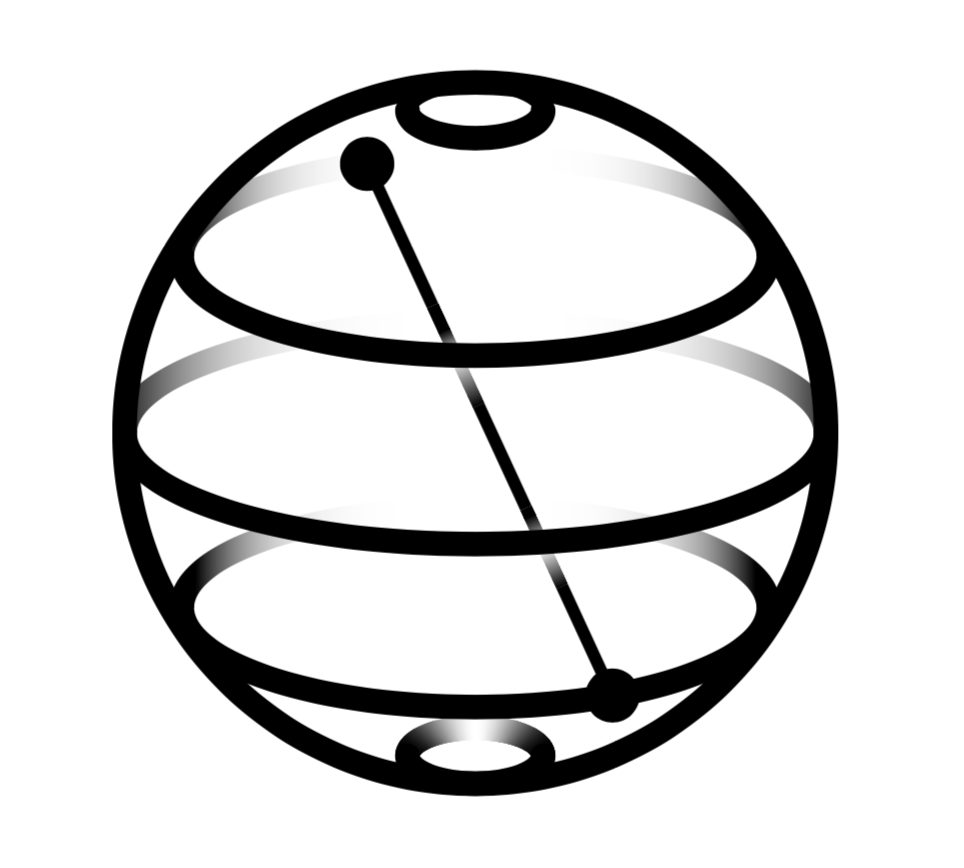
\includegraphics[width=\textwidth]{qiskit_logo.png}
    \end{columns}
\end{frame}

\begin{frame}
    \frametitle{Qiskit Elements}
    \centering
    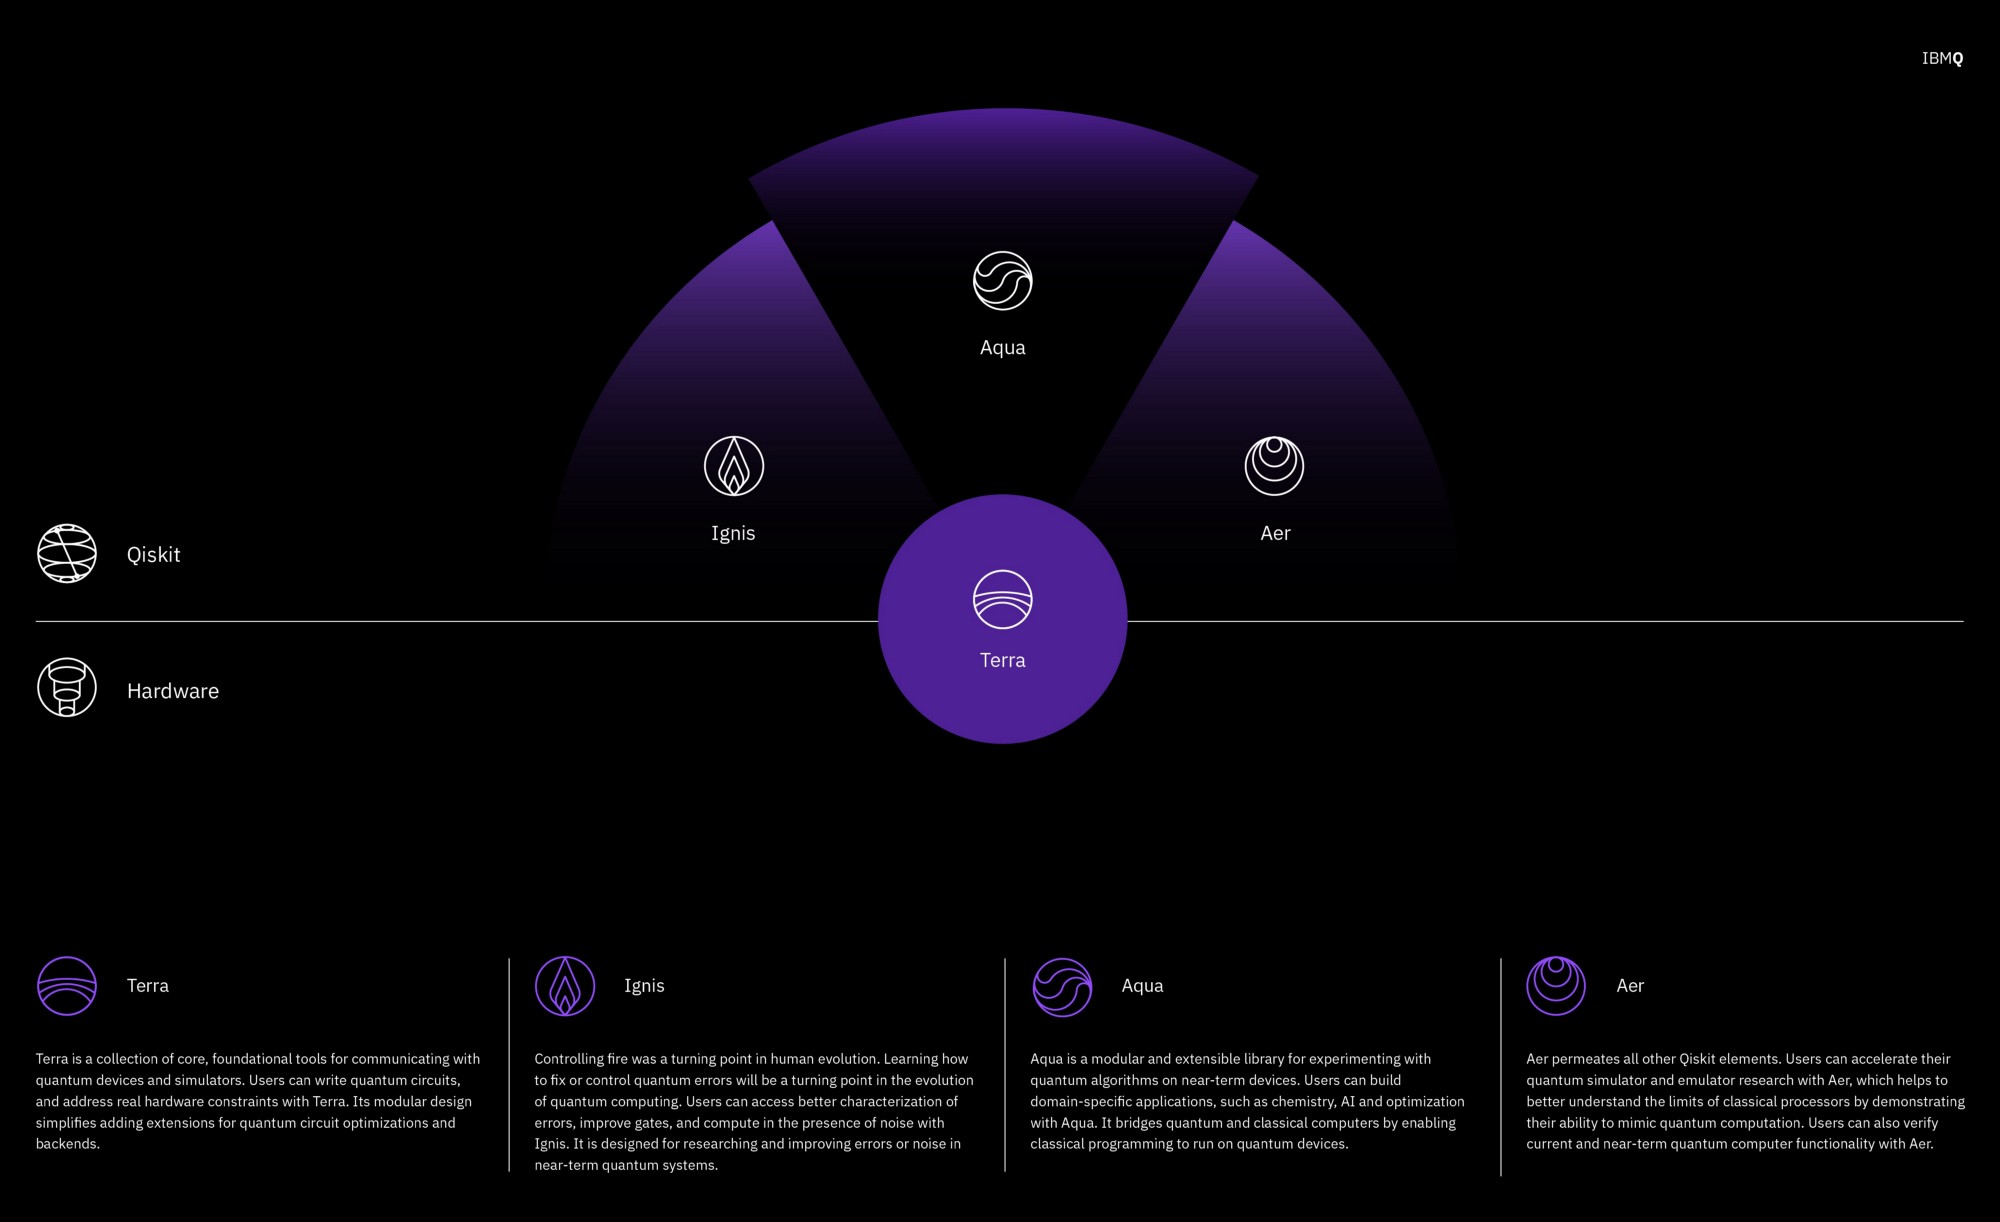
\includegraphics[width=.99\textwidth]{qiskit-components.jpeg}
\end{frame}

\begin{frame}
    \frametitle{Qiskit Terra}
    \begin{columns}
        \column{.5\textwidth}
           \begin{itemize}
                \item Is the base layer for applications, provides interface to hardware and simulators
                \item Provides an SDK for working with quantum circuits
                \item Compiles circuits to run on different backends
                \item Written in Python
           \end{itemize}
        \column{.5\textwidth}
            \centering
            \colorbox{black}{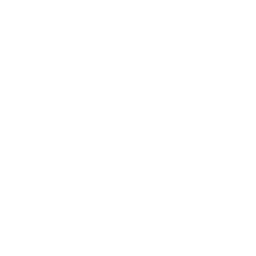
\includegraphics[width=.5\textwidth]{qiskit-terra-logo.png}}
    \end{columns}
\end{frame}

\section{Quantum Information Theory}
\subsection{The Qubit}
\begin{frame}
    \frametitle{The Qubit}
    \begin{columns}
        \column{.4\textwidth}
            \begin{itemize}
                \item The bloch sphere provides a representation of qubit state
                \item State can be at any point along surface of sphere
                \item Measuring a qubit occurs along the Z axis. (also called basis states)
                \item Measuring a qubit is irreversible and will either be 0
                      or 1
            \end{itemize}
        \column{.6\textwidth}
            \begin{center}
                \textbf{Bloch Sphere:}
                \only<1>{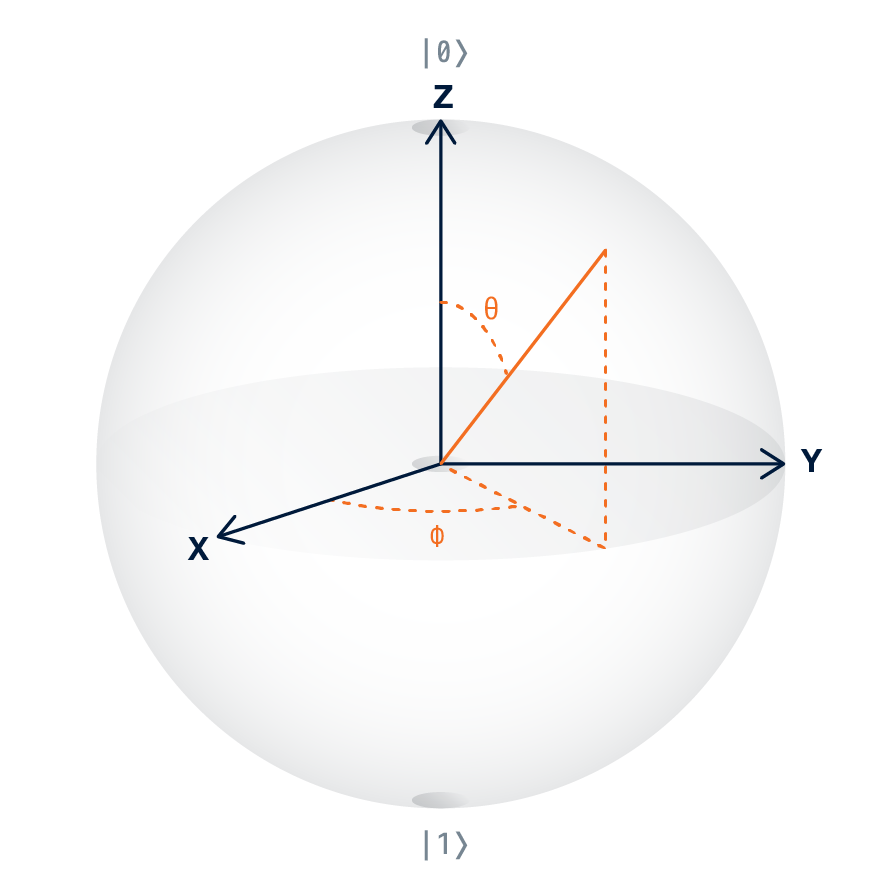
\includegraphics[height=.85\textheight]{bloch_angles.png}}
                \only<2>{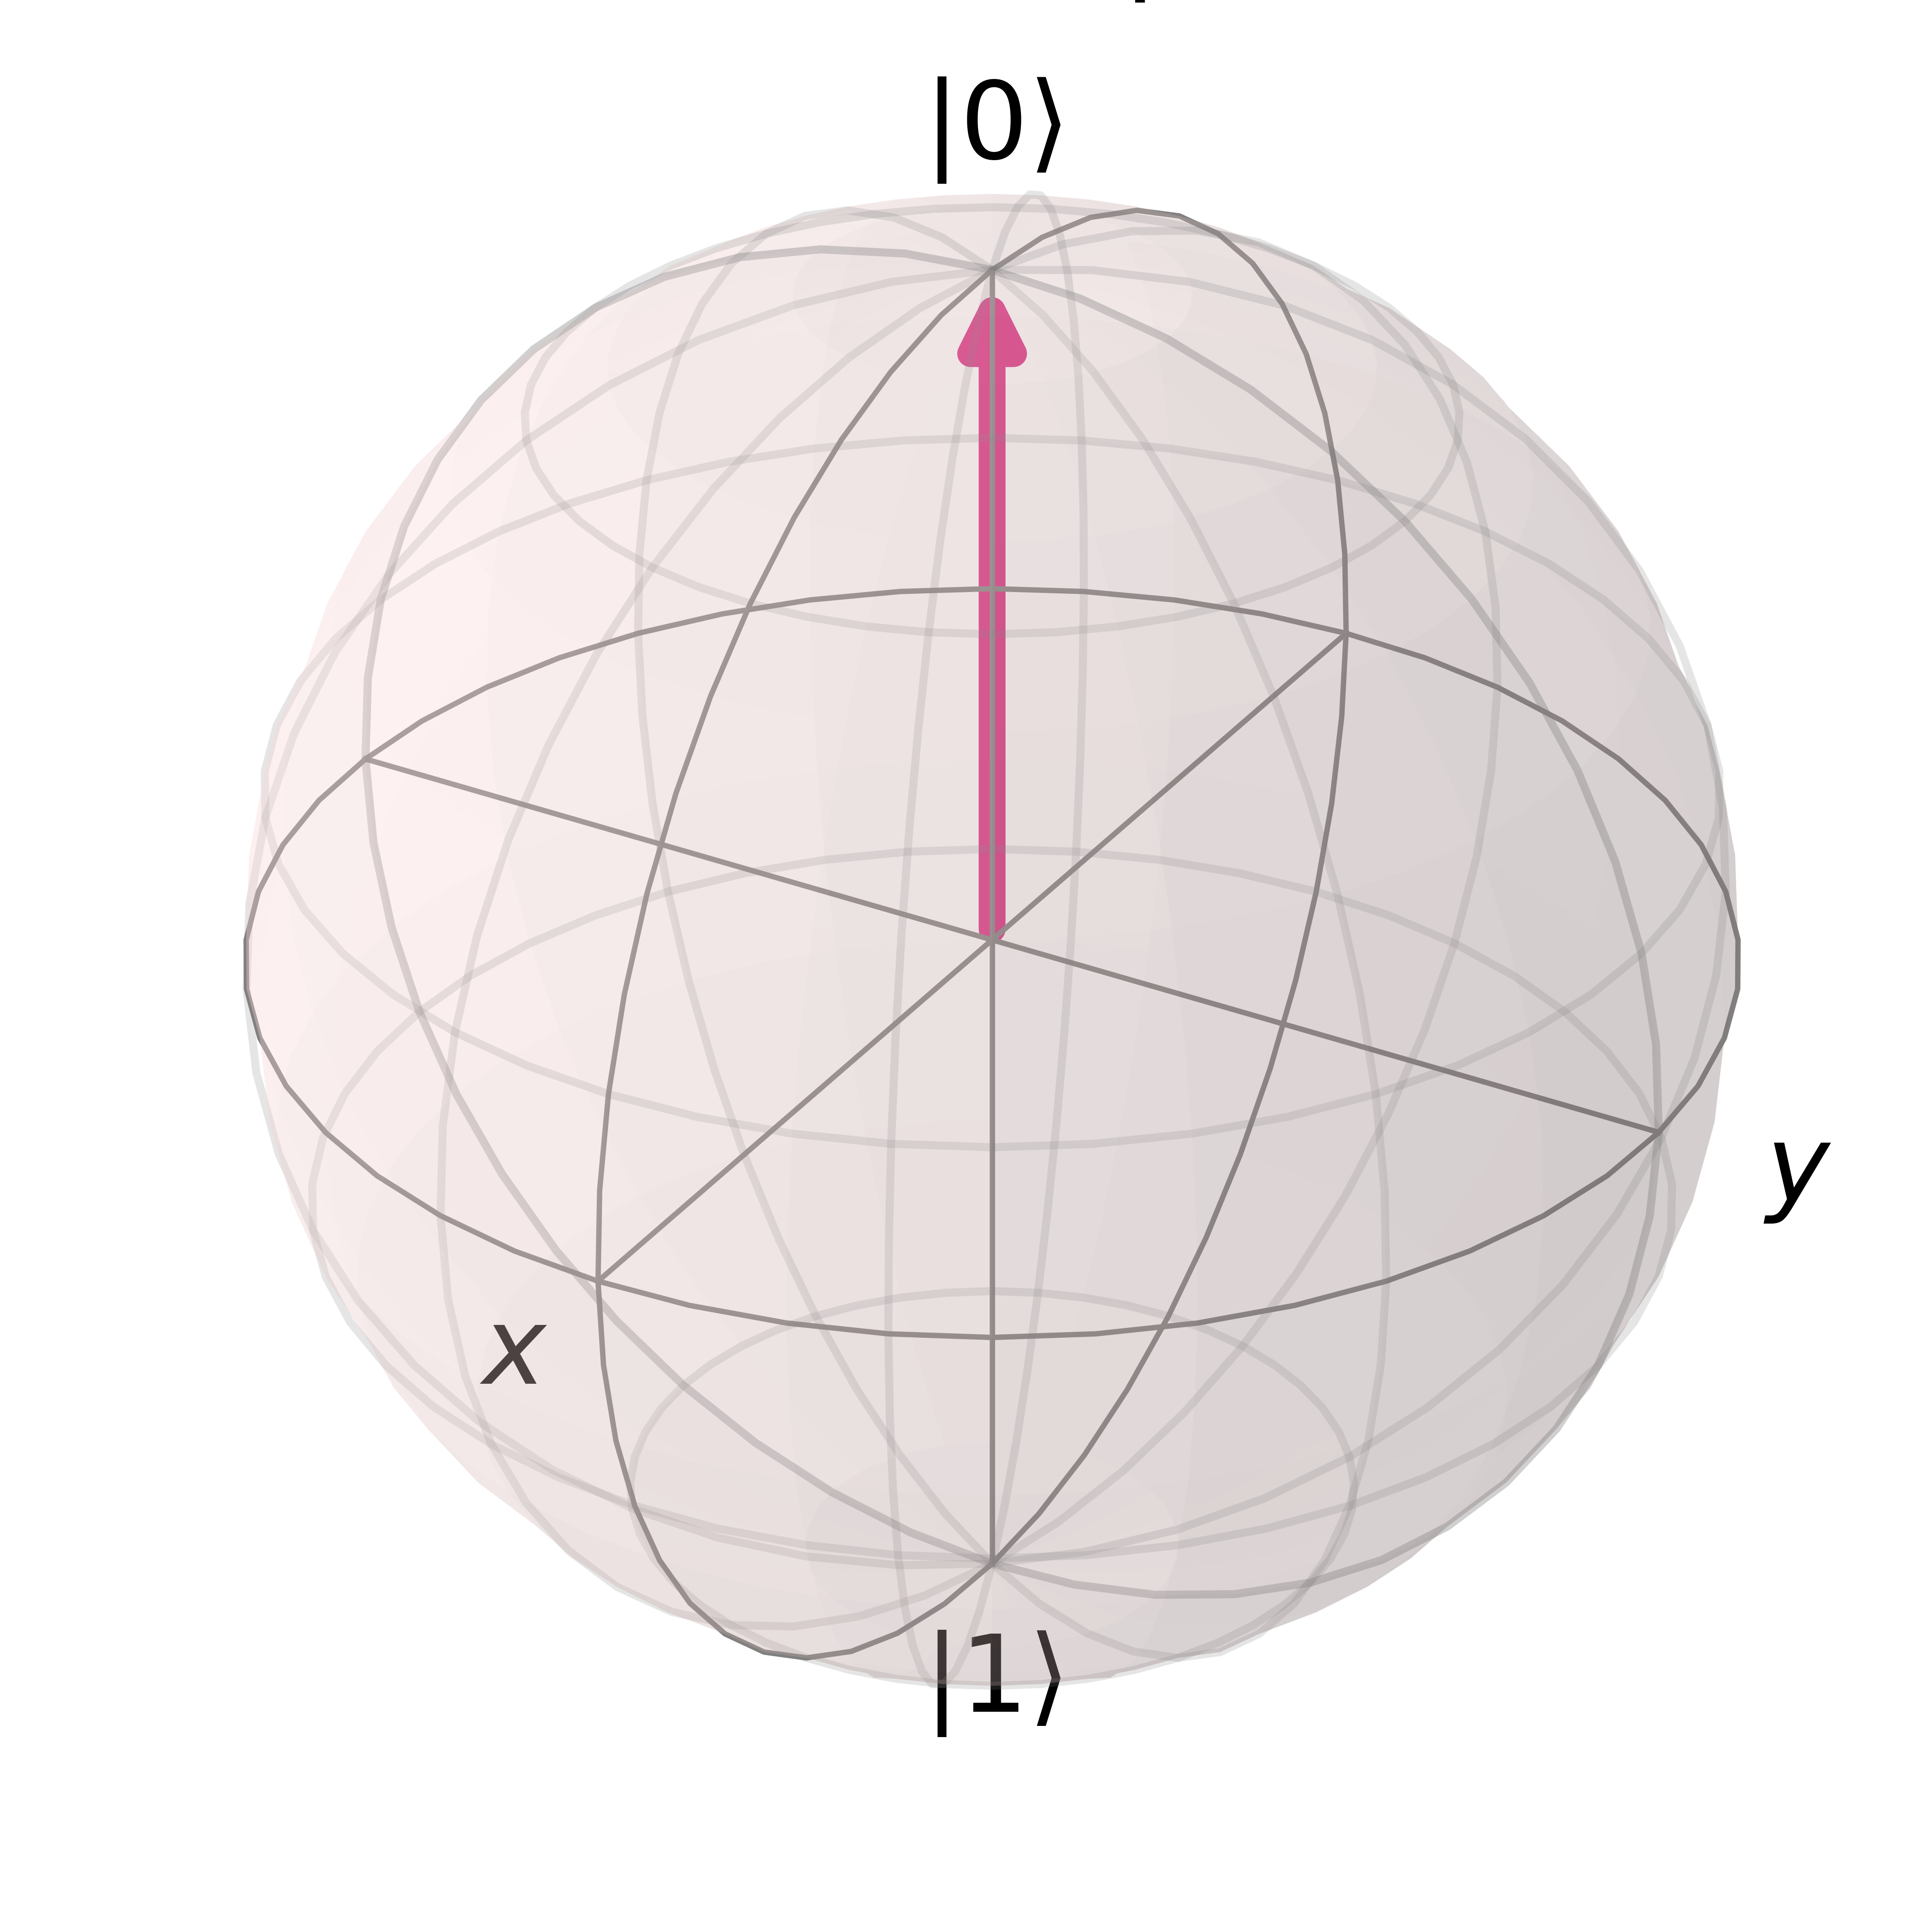
\includegraphics[height=.85\textheight]{bloch_fresh.png}}
                \only<3>{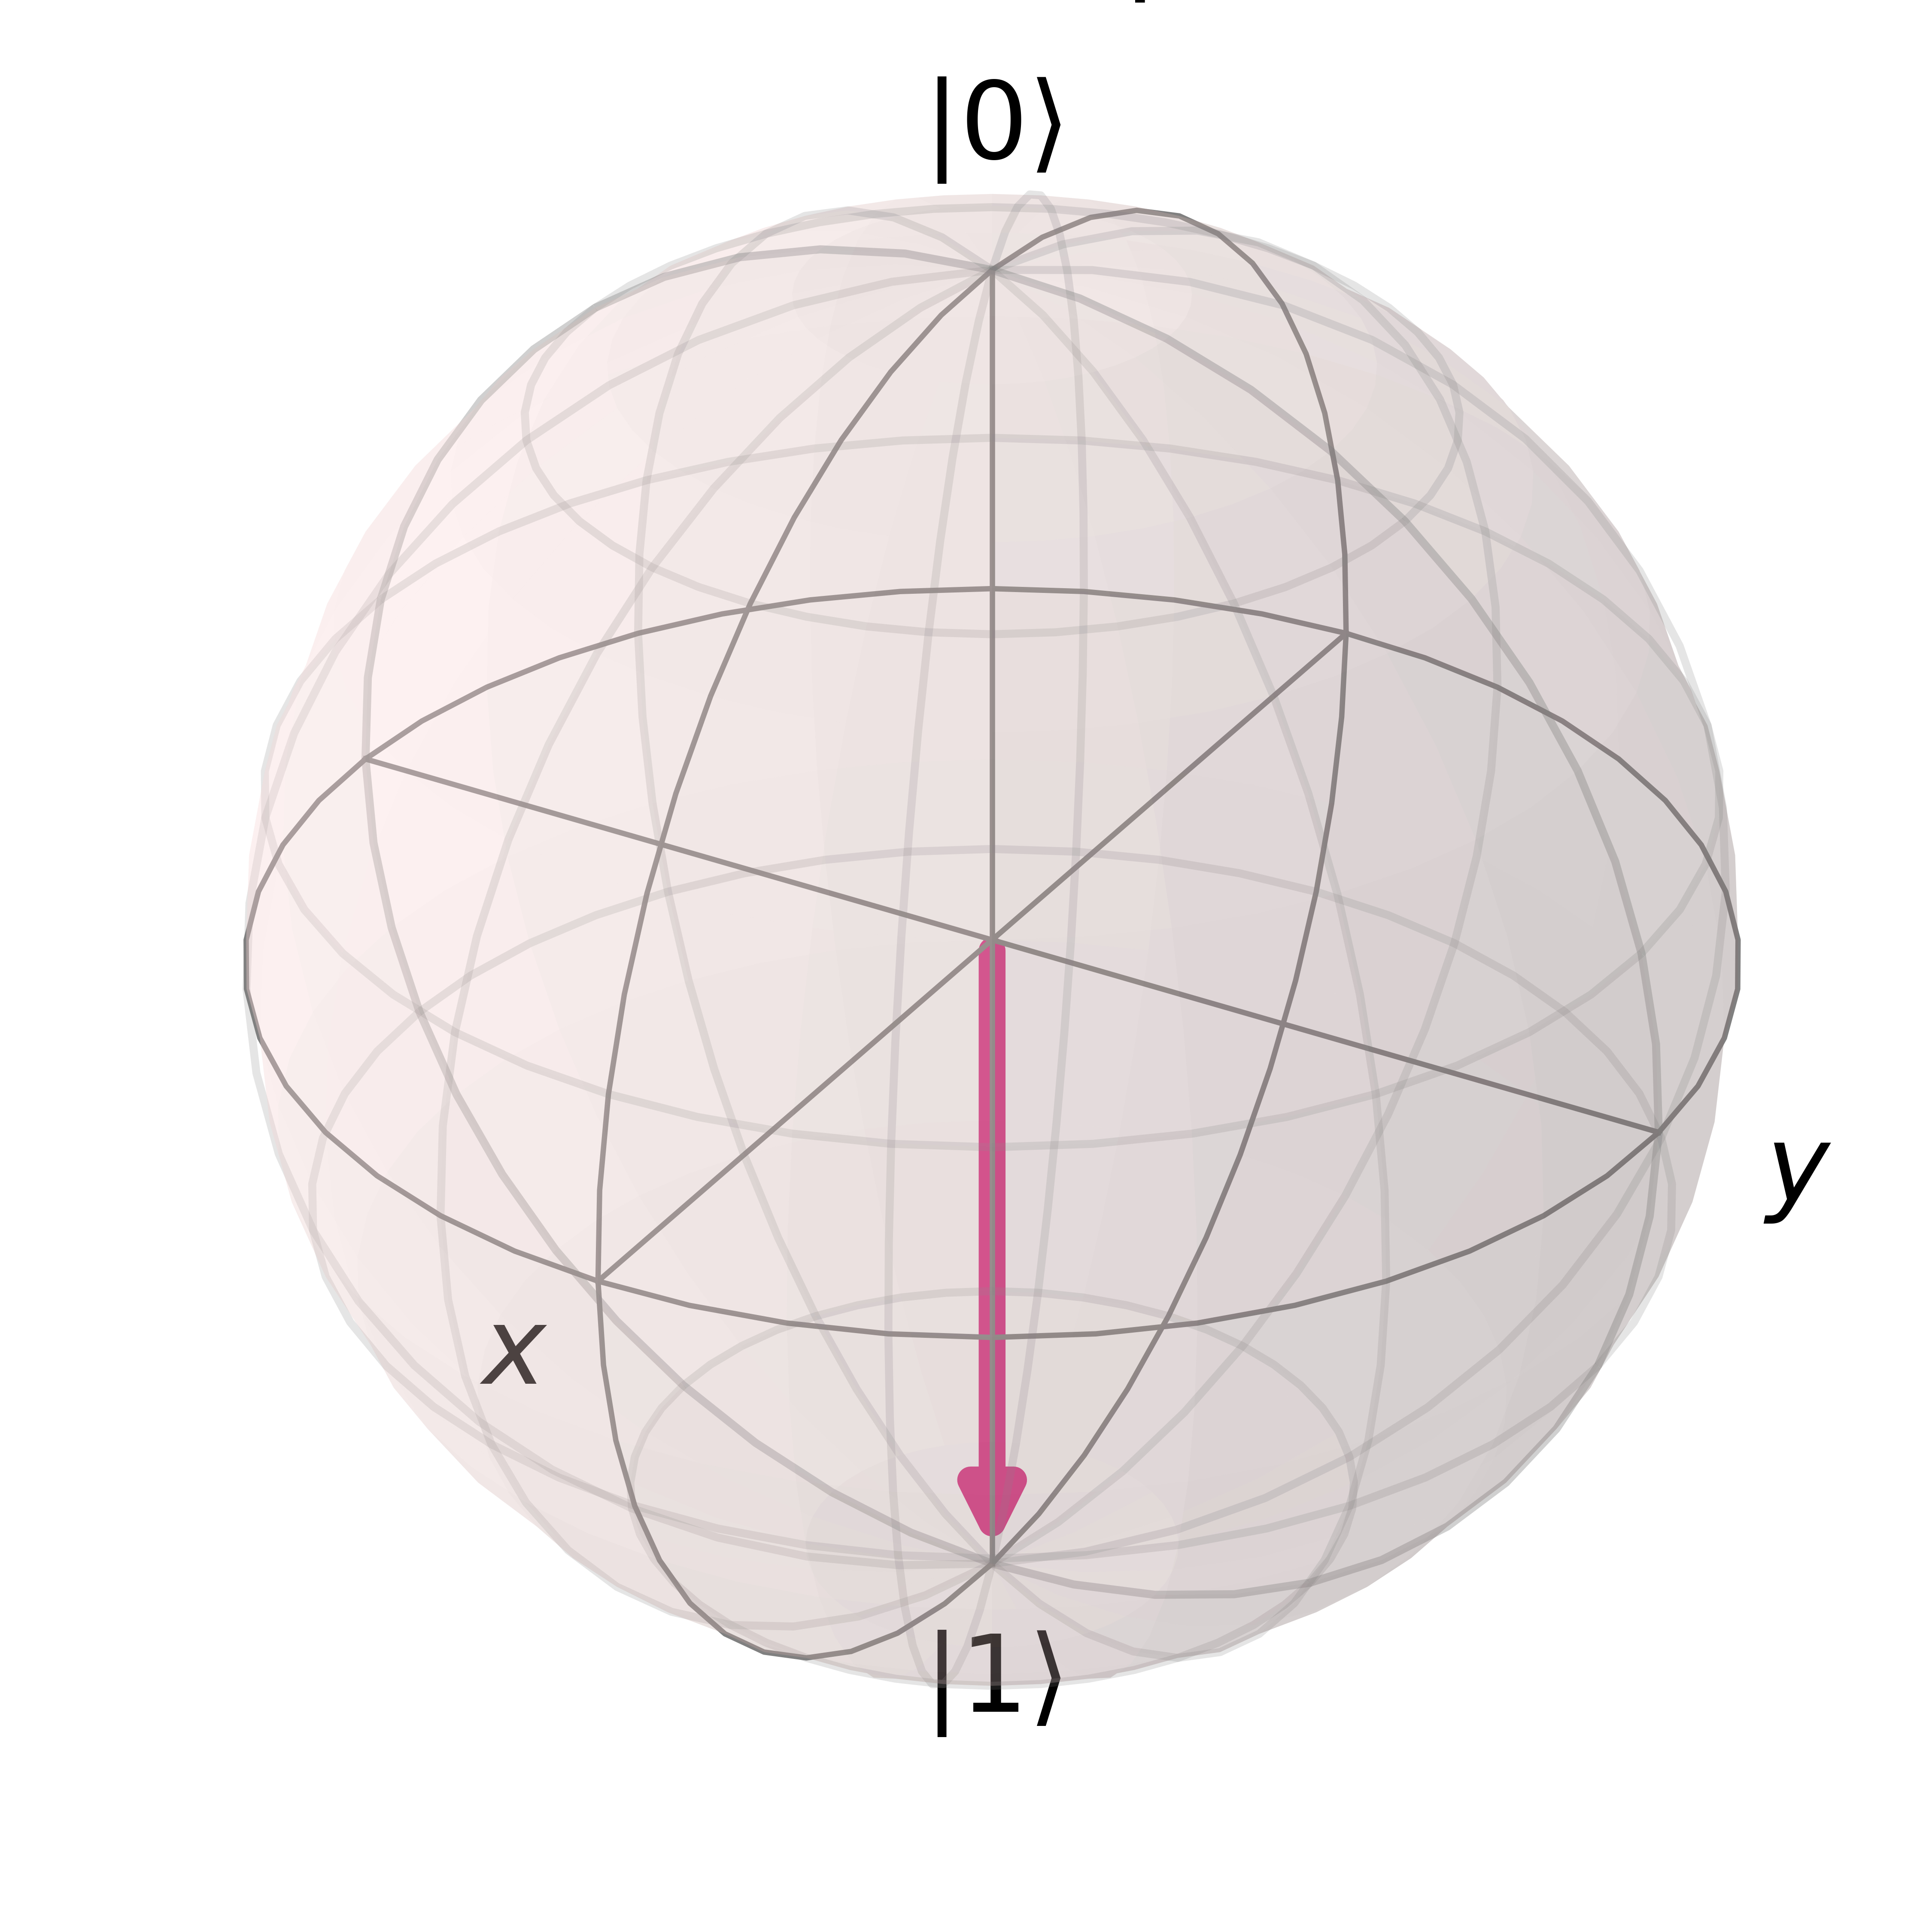
\includegraphics[height=.85\textheight]{bloch_one.png}}
        \end{center}
    \end{columns}
\end{frame}

\subsection{Quantum Gates}
\begin{frame}
    \frametitle{Quantum Gates}
    \begin{itemize}  
        \item Quantum Logic Gates are used perform operations on qubits
        \item Gates are reversible
        \item Gates can be represented as unitary matrices
    \end{itemize}
    \centering
    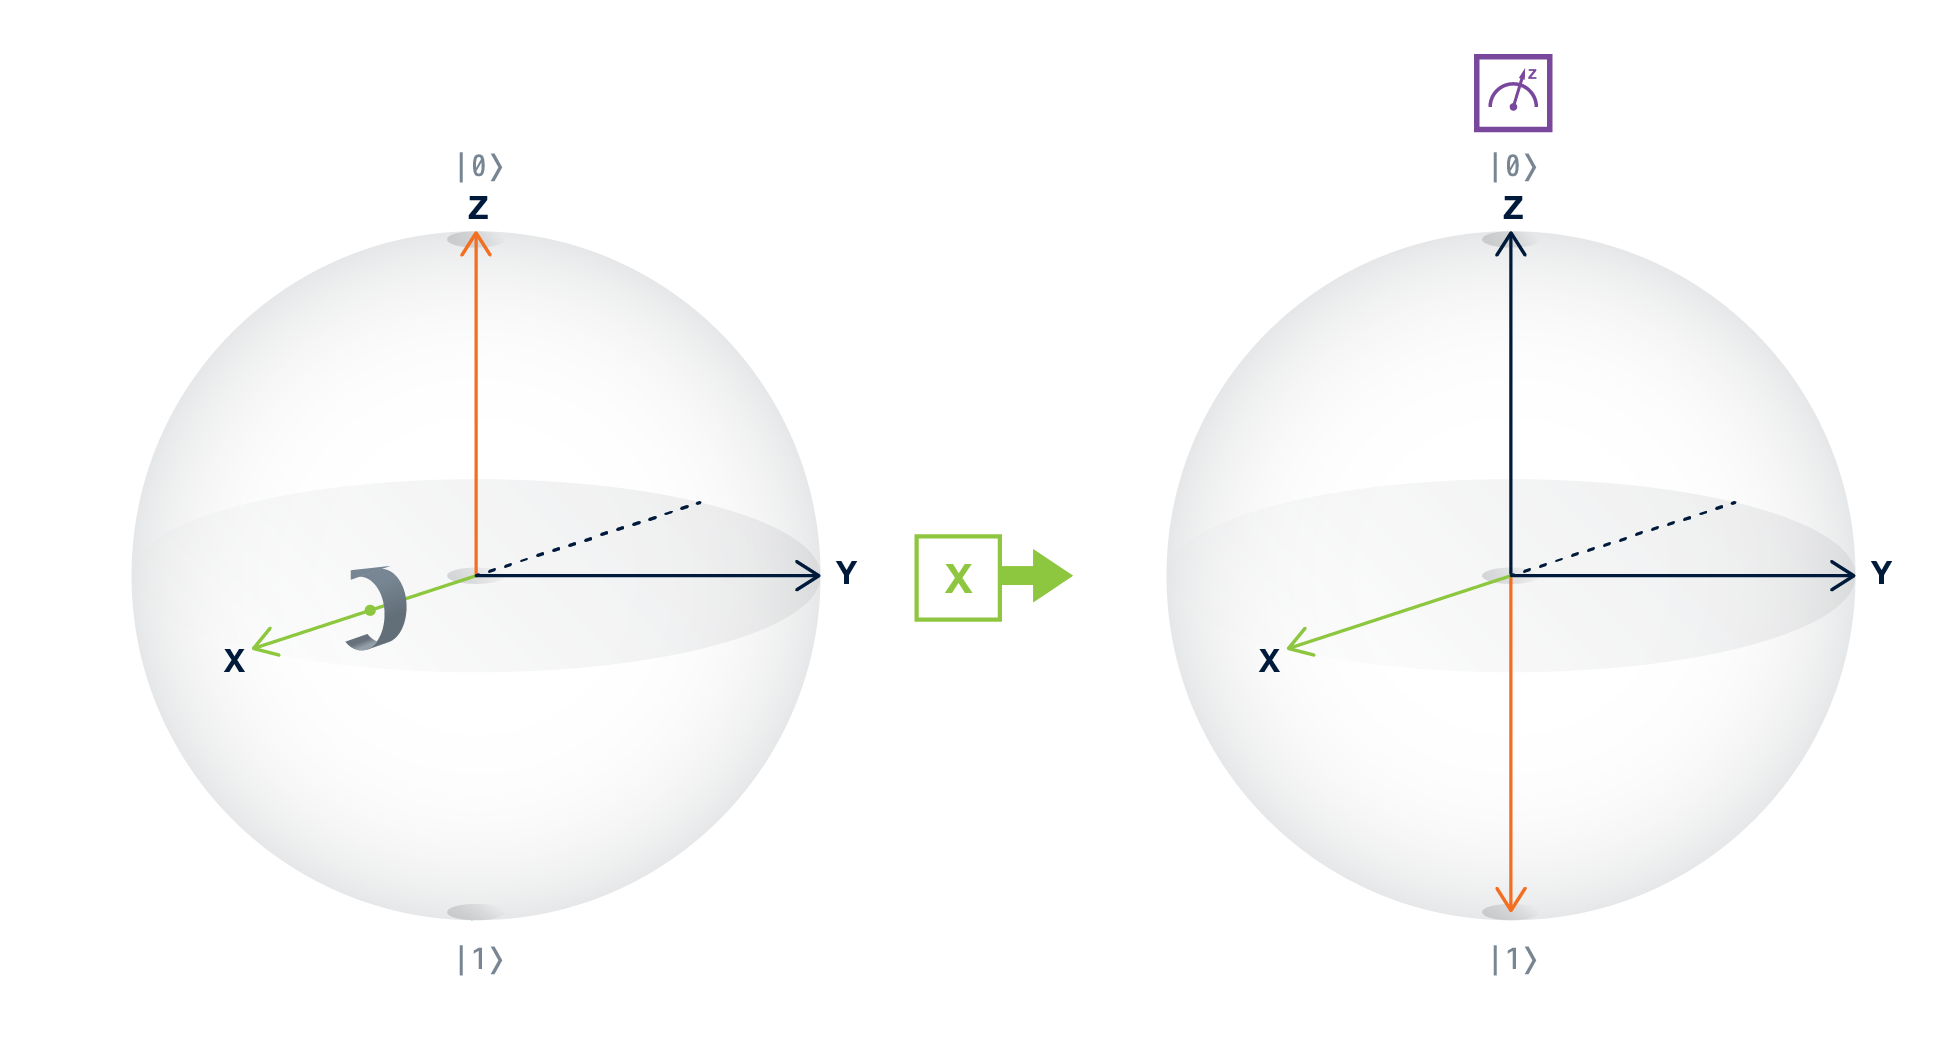
\includegraphics[width=.9\textwidth]{gate_x_bloch.png}
%    \begin{columns}[onlytextwidth]
%        \begin{column}{.333\textwidth}
%            \centering
%            \textbf{Gate}
%            \begin{equation*}
%                \Qcircuit @C=0.5em @R=0.0em @!R {
%	 	            \lstick{\ket{0}} & \gate{X} & \qw & \qw\\
%            	}
%            \end{equation*} \\
%        \end{column}
%        \begin{column}{.333\textwidth}
%            \centering
%            \textbf{Matrix Form}
%            \[\begin{bmatrix}
%                0 & 1\\
%                1 & 0 \\
%            \end{bmatrix}\]\\
%        \end{column}
%    \end{columns}
\end{frame}

\subsection{CNOT Gate}
\begin{frame}
    \frametitle{Controlled Not Gate}
    \centering
    \textbf{CNOT flips the \textit{target} bit if the \textit{control} bit is 1}
    \begin{equation*}
        \Qcircuit {
            \lstick{\ket{0}}  & \ctrl{1} & \rstick{\ket{0}} \qw \\ 
            \lstick{a\ket{0} + b\ket{1}} &  \targ & \rstick{a\ket{0} + b\ket{1}} \qw \\
    }
    \end{equation*}\\
    \vspace{3em}
    \begin{equation*}
        \Qcircuit {
            \lstick{\ket{1}} & \ctrl{1} & \rstick{\ket{1}} \qw\\ 
            \lstick{a\ket{0} + b\ket{1}} & \targ & \rstick{b\ket{0} + a\ket{1}} \qw\\
    }
    \end{equation*}
\end{frame}

\subsection{Quantum Circuits}
\begin{frame}
    \frametitle{Quantum Circuits}
    \textbf{Putting it together you build a circuit like:}
    \begin{equation*}
        \Qcircuit @C=0.5em @R=0.0em @!R {
            \lstick{q0_{2}: \ket{0}} & \gate{X} & \gate{H} & \ctrl{2} &\qw & \meter & \qw & \qw & \qw & \qw\\
        \lstick{q0_{1}: \ket{0}} & \gate{X} & \gate{H} & \qw & \qw & \qw & \meter & \qw & \qw\\
        \lstick{q0_{0}: \ket{0}} & \qw & \gate{H} & \targ &  \qw & \qw & \qw & \meter & \qw & \qw\\
	 	\lstick{c0_{2}: 0} & \cw & \cw & \cw & \cw & \cw \cwx[-3] & \cw & \cw & \cw & \cw\\
	 	\lstick{c0_{1}: 0} & \cw & \cw & \cw & \cw & \cw & \cw \cwx[-3] & \cw & \cw & \cw\\
	 	\lstick{c0_{0}: 0} & \cw & \cw & \cw & \cw & \cw & \cw & \cw \cwx[-3] & \cw & \cw\\
	 }
    \end{equation*}
    \begin{itemize}
        \item Each row represents a bit, either quantum or classical
        \item The operations are performed each qubit left to right
        \item Shows dependencies of operations
    \end{itemize}
\end{frame}

\begin{frame}
    \frametitle{Superposition and Entanglement}
    There are 2 key properties of Quantum Mechanics that are fundamental to
    Quantum Computing:
    \begin{enumerate}
        \item A physical system in a definite state can still behave randomly.
        \item Two systems that are too far apart to influence each other can
              nevertheless behave in ways that, though individually random,
              are somehow strongly correlated.
    \end{enumerate}
\end{frame}

\subsection{Superposition and Hadamards}
\begin{frame}
    \frametitle{Superposition}
    \begin{itemize}
    \item Identically prepared qubits can still behave randomly
    \item The randomness is inherent in nature
    \end{itemize}
    \begin{columns}
        \column{.5\textwidth}
            \centering
            \LARGE \textbf{$\ket{0}$} \\
            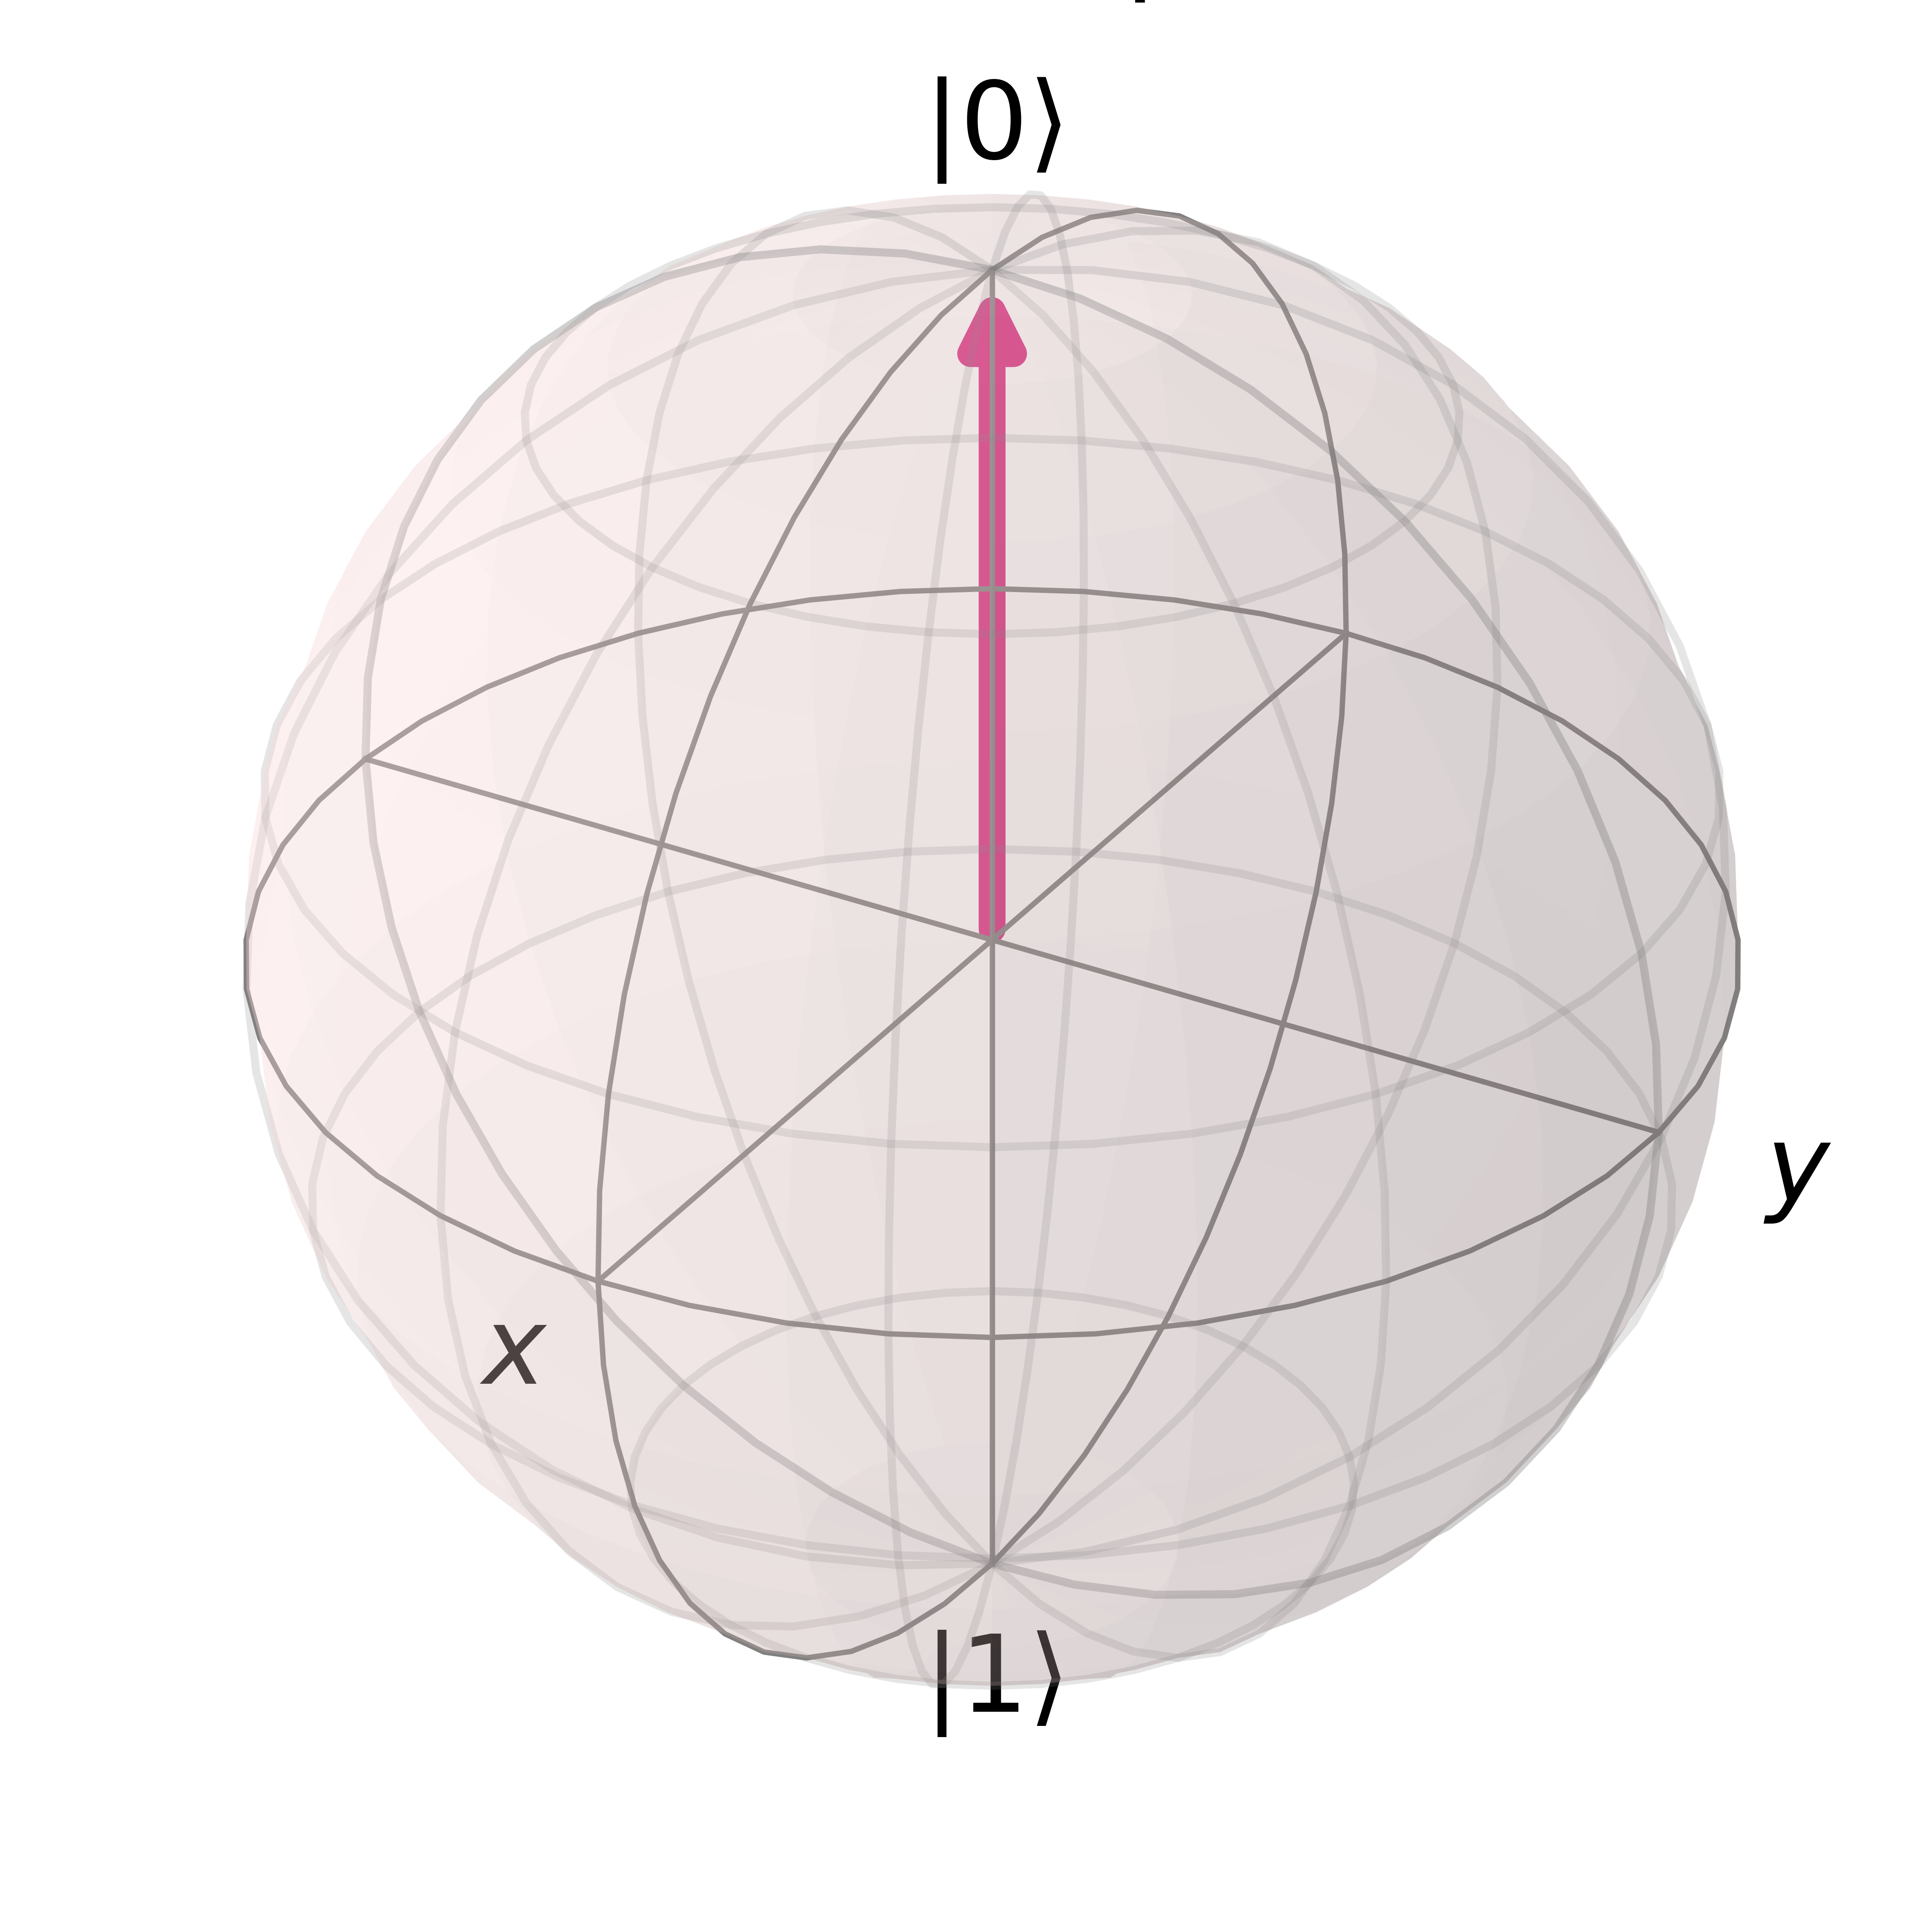
\includegraphics[width=.4\textwidth]{bloch_fresh.png} \\
            \LARGE \textbf{$\ket{1}$} \\
            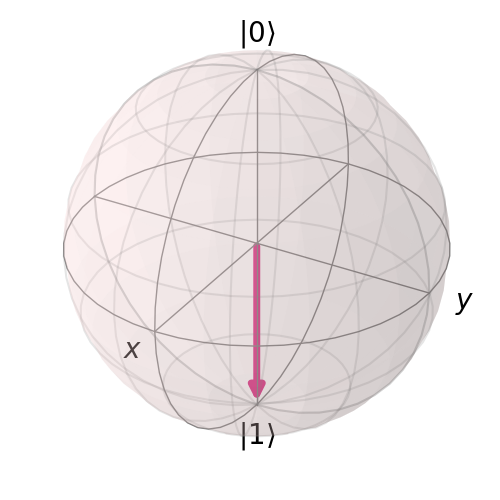
\includegraphics[width=.4\textwidth]{bloch_x.png}\\
        \column{.5\textwidth}
            \centering
            \LARGE \textbf{$\ket{0} + \ket{1}$} \\
            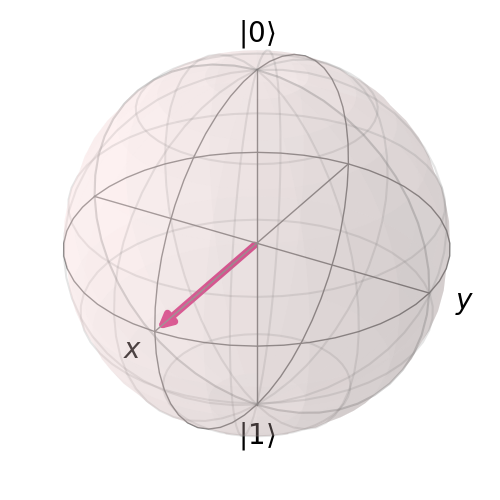
\includegraphics[width=.5\textwidth]{bloch_hadamard.png}\\
            \textbf{$\sim$50/50 chance of being \ket{0} or \ket{1}}
    \end{columns}
\end{frame}

\begin{frame}
    \frametitle{Hadamard Gate}
%    \begin{columns}
%        \column{.5\textwidth}
%        \centering
%        \textbf{Gate}
%        \begin{equation*}
%            \Qcircuit @C=0.5em @R=0.0em @!R {
%	 	        \lstick{\ket{0}} & \gate{H} & \qw & \qw\\
%    	     }
%        \end{equation*}
%        \column{.5\textwidth}
%        \centering
%        \textbf{Matrix Form}
%        \[\frac{1}{\sqrt{2}} \begin{bmatrix}
%            1 & 1 \\
%            1 & -1 \\
%        \end{bmatrix}\]
%    \end{columns}
    \centering
    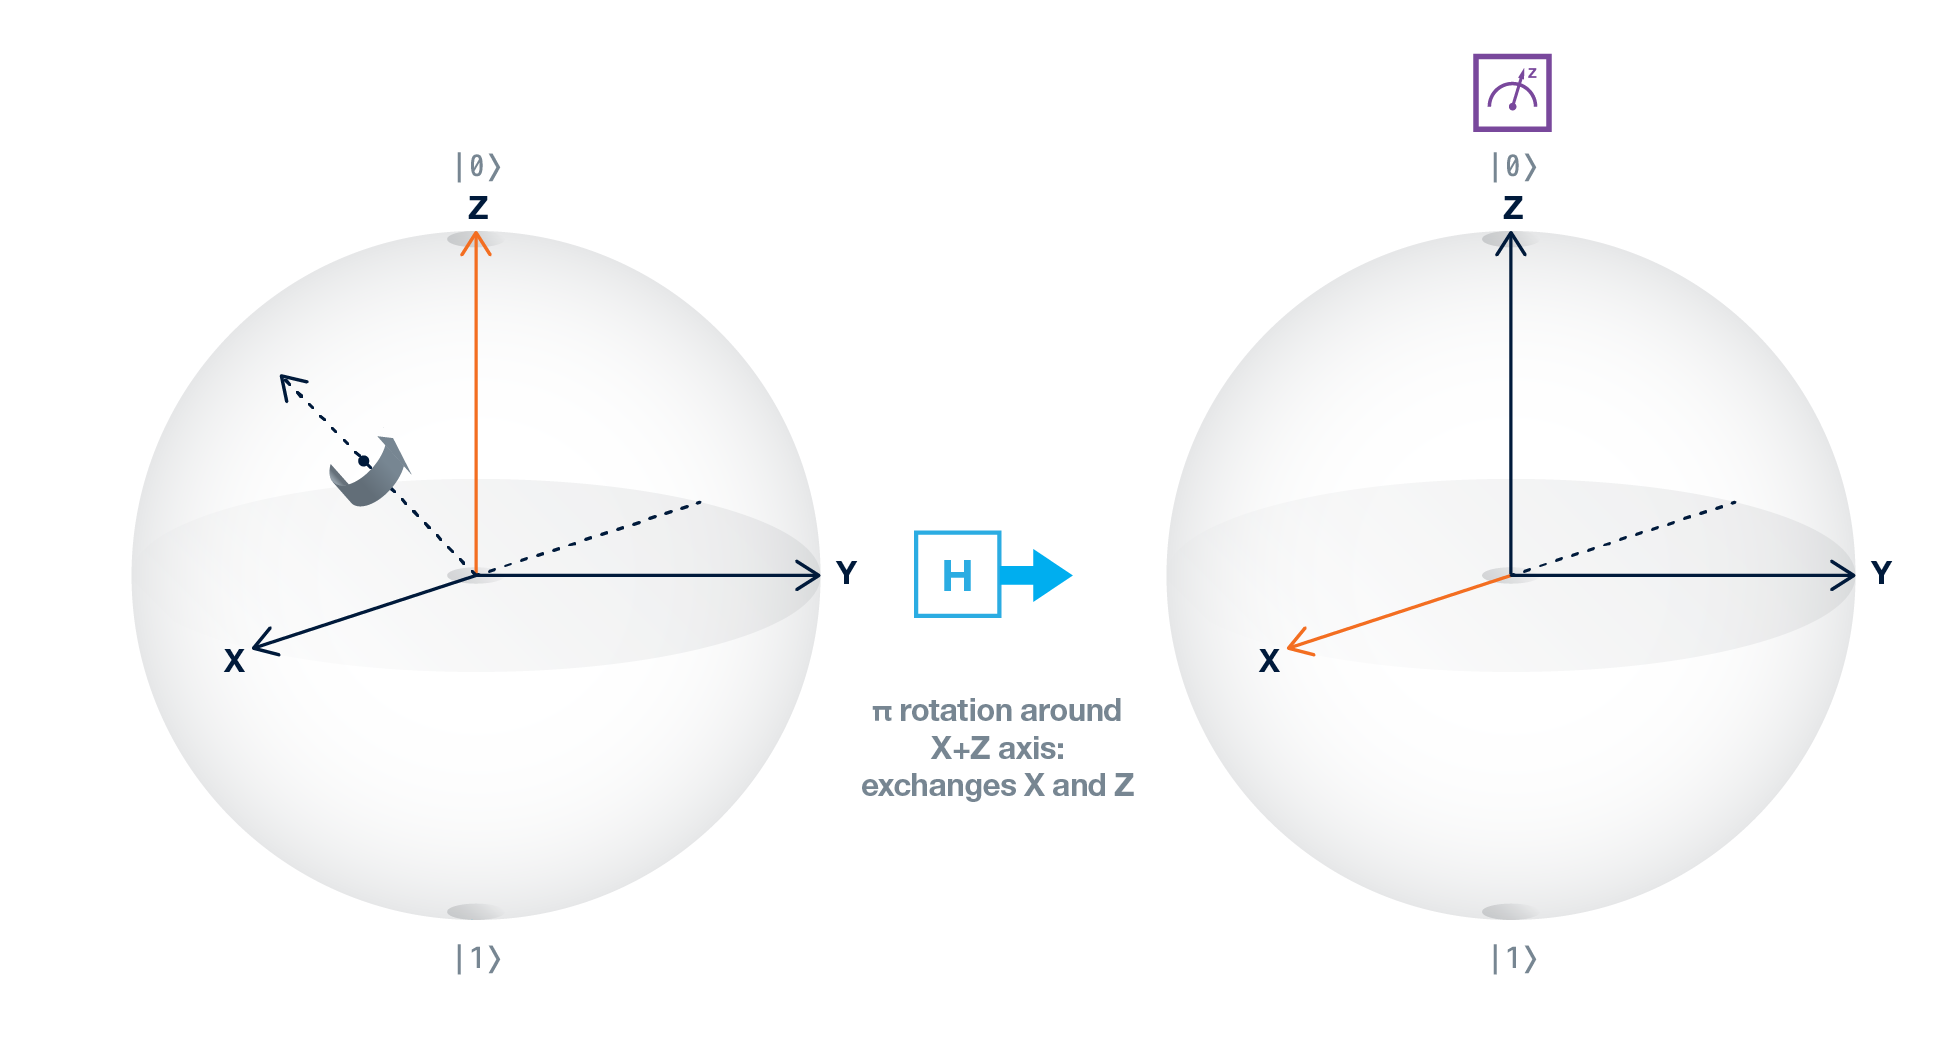
\includegraphics[width=\textwidth]{gate_h_bloch.png}
\end{frame}

\begin{frame}
    \frametitle{Qubit Phase}
    \begin{columns}
    \column{.4\textwidth}
        \begin{itemize}
            \item While qubits are read along the basis vectors you can
                still use the other dimensions
            \item The phase can be leveraged to encode more information in the qubit
        \end{itemize}
        \column{.6\textwidth}
            \centering
            \textbf{Phase is $\phi$:}
            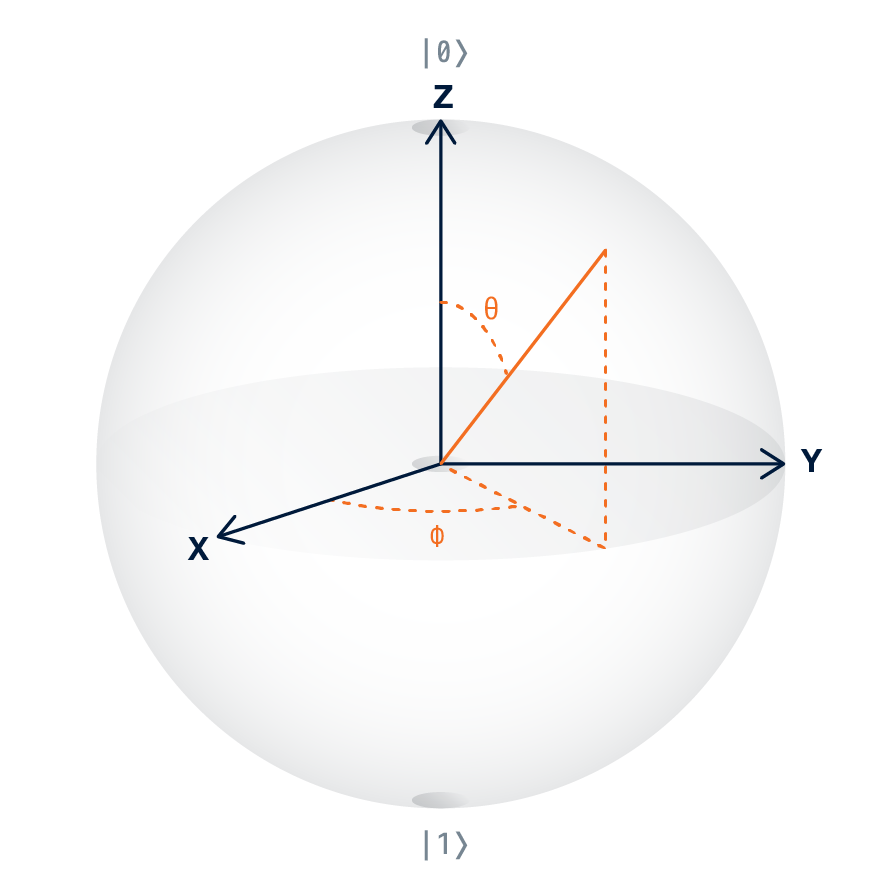
\includegraphics[height=.85\textwidth]{bloch_angles.png}
    \end{columns}
\end{frame}

\begin{frame}
    \frametitle{Hadamard and Phase}
    \textbf{Hadamard gates are self inverses:}
    \centering
    \only<1> {
        \begin{equation*}
            \Qcircuit {
                \lstick{\ket{0}} & \gate{H} & \qw & \mbox{\ket{0} + \ket{1}} & \hspace{5em} & \gate{H} & \rstick{\ket{0}} \qw
        }
        \end{equation*} \\
        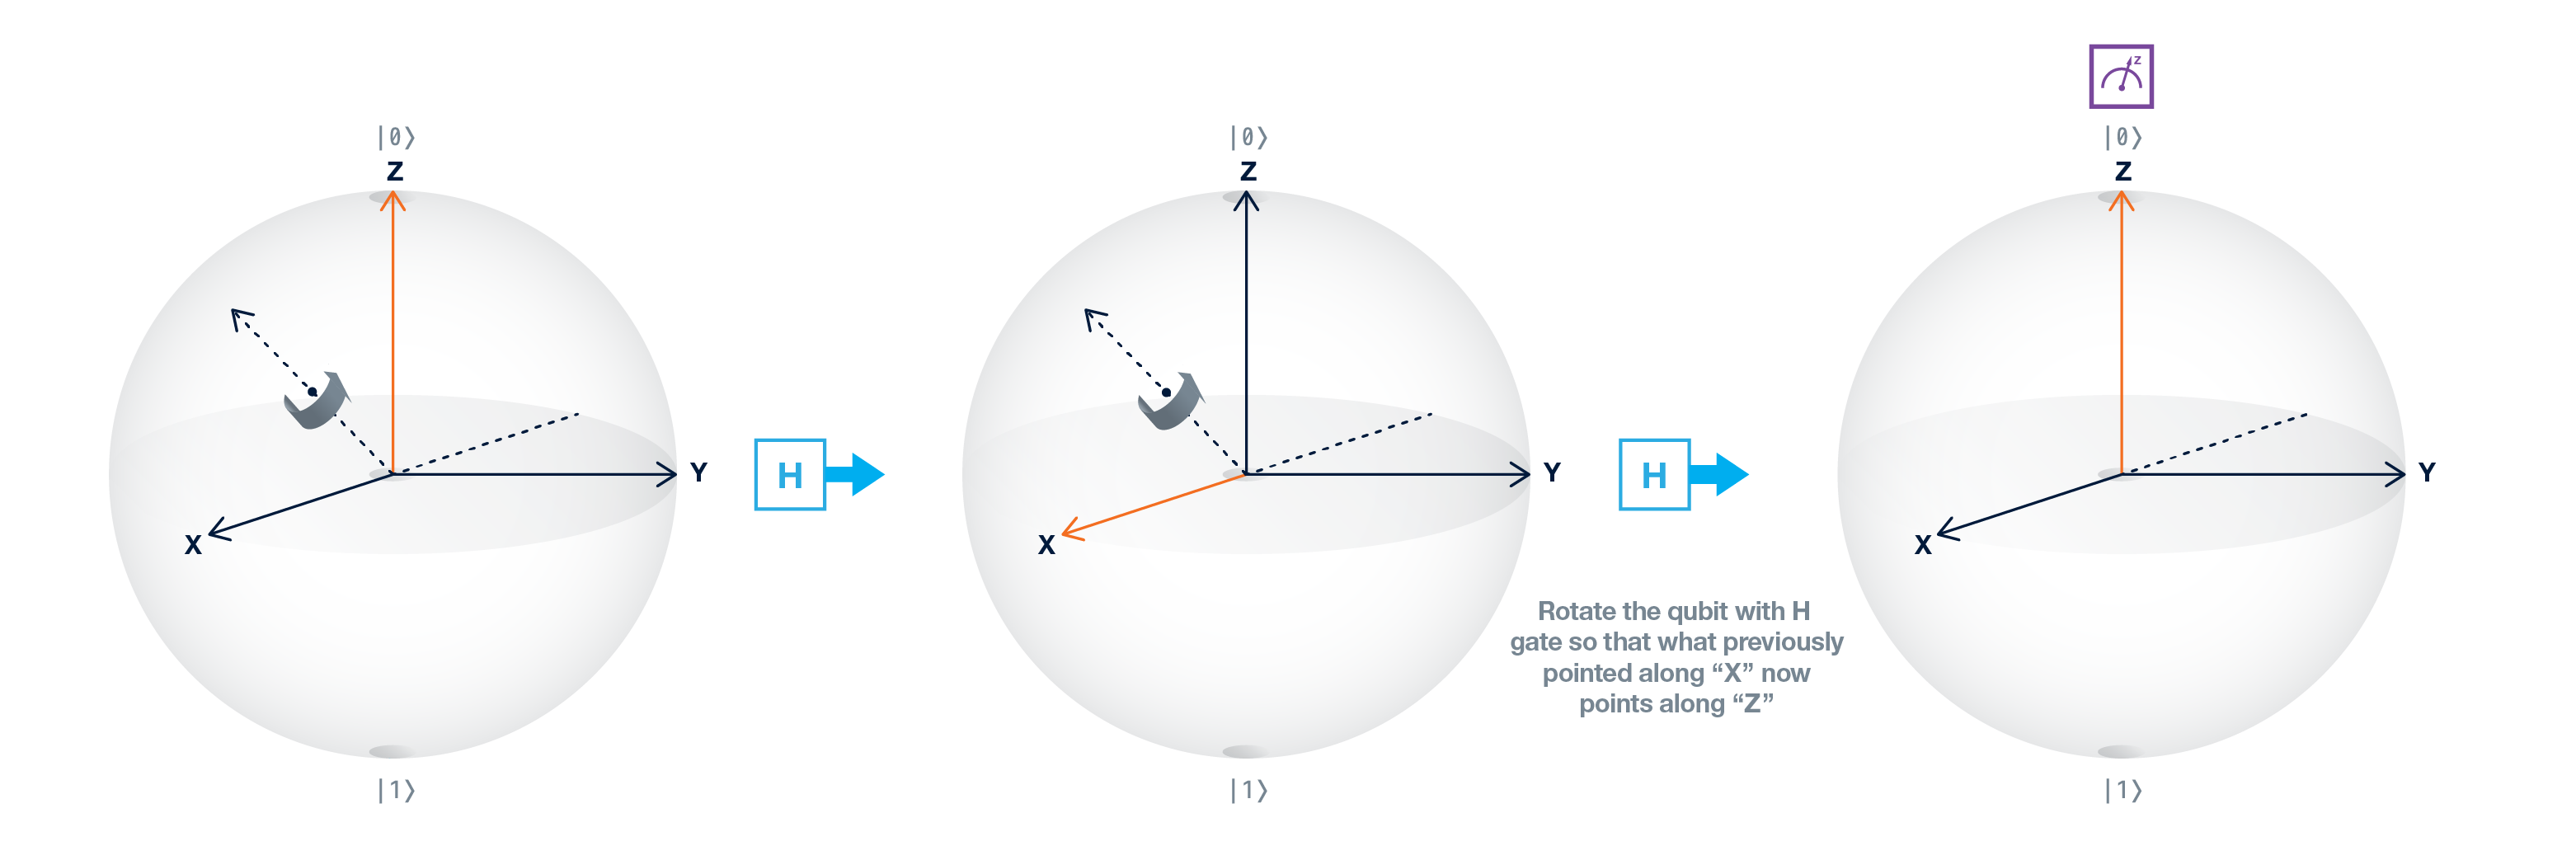
\includegraphics[width=\textwidth]{double_h_gate_bloch.png}
    }
    \only<2> {
        \begin{equation*}
            \Qcircuit {
                \lstick{\ket{1}} & \gate{H} & \qw & \mbox{\ket{0} {\color{red} \textbf{-}} \ket{1}} & \hspace{5em} & \gate{H} & \rstick{\ket{1}} \qw \\
                & & & \mbox{\color{red} Phase} & & &
            }
        \end{equation*}
        \begin{columns}
            \column{.5\textwidth}
            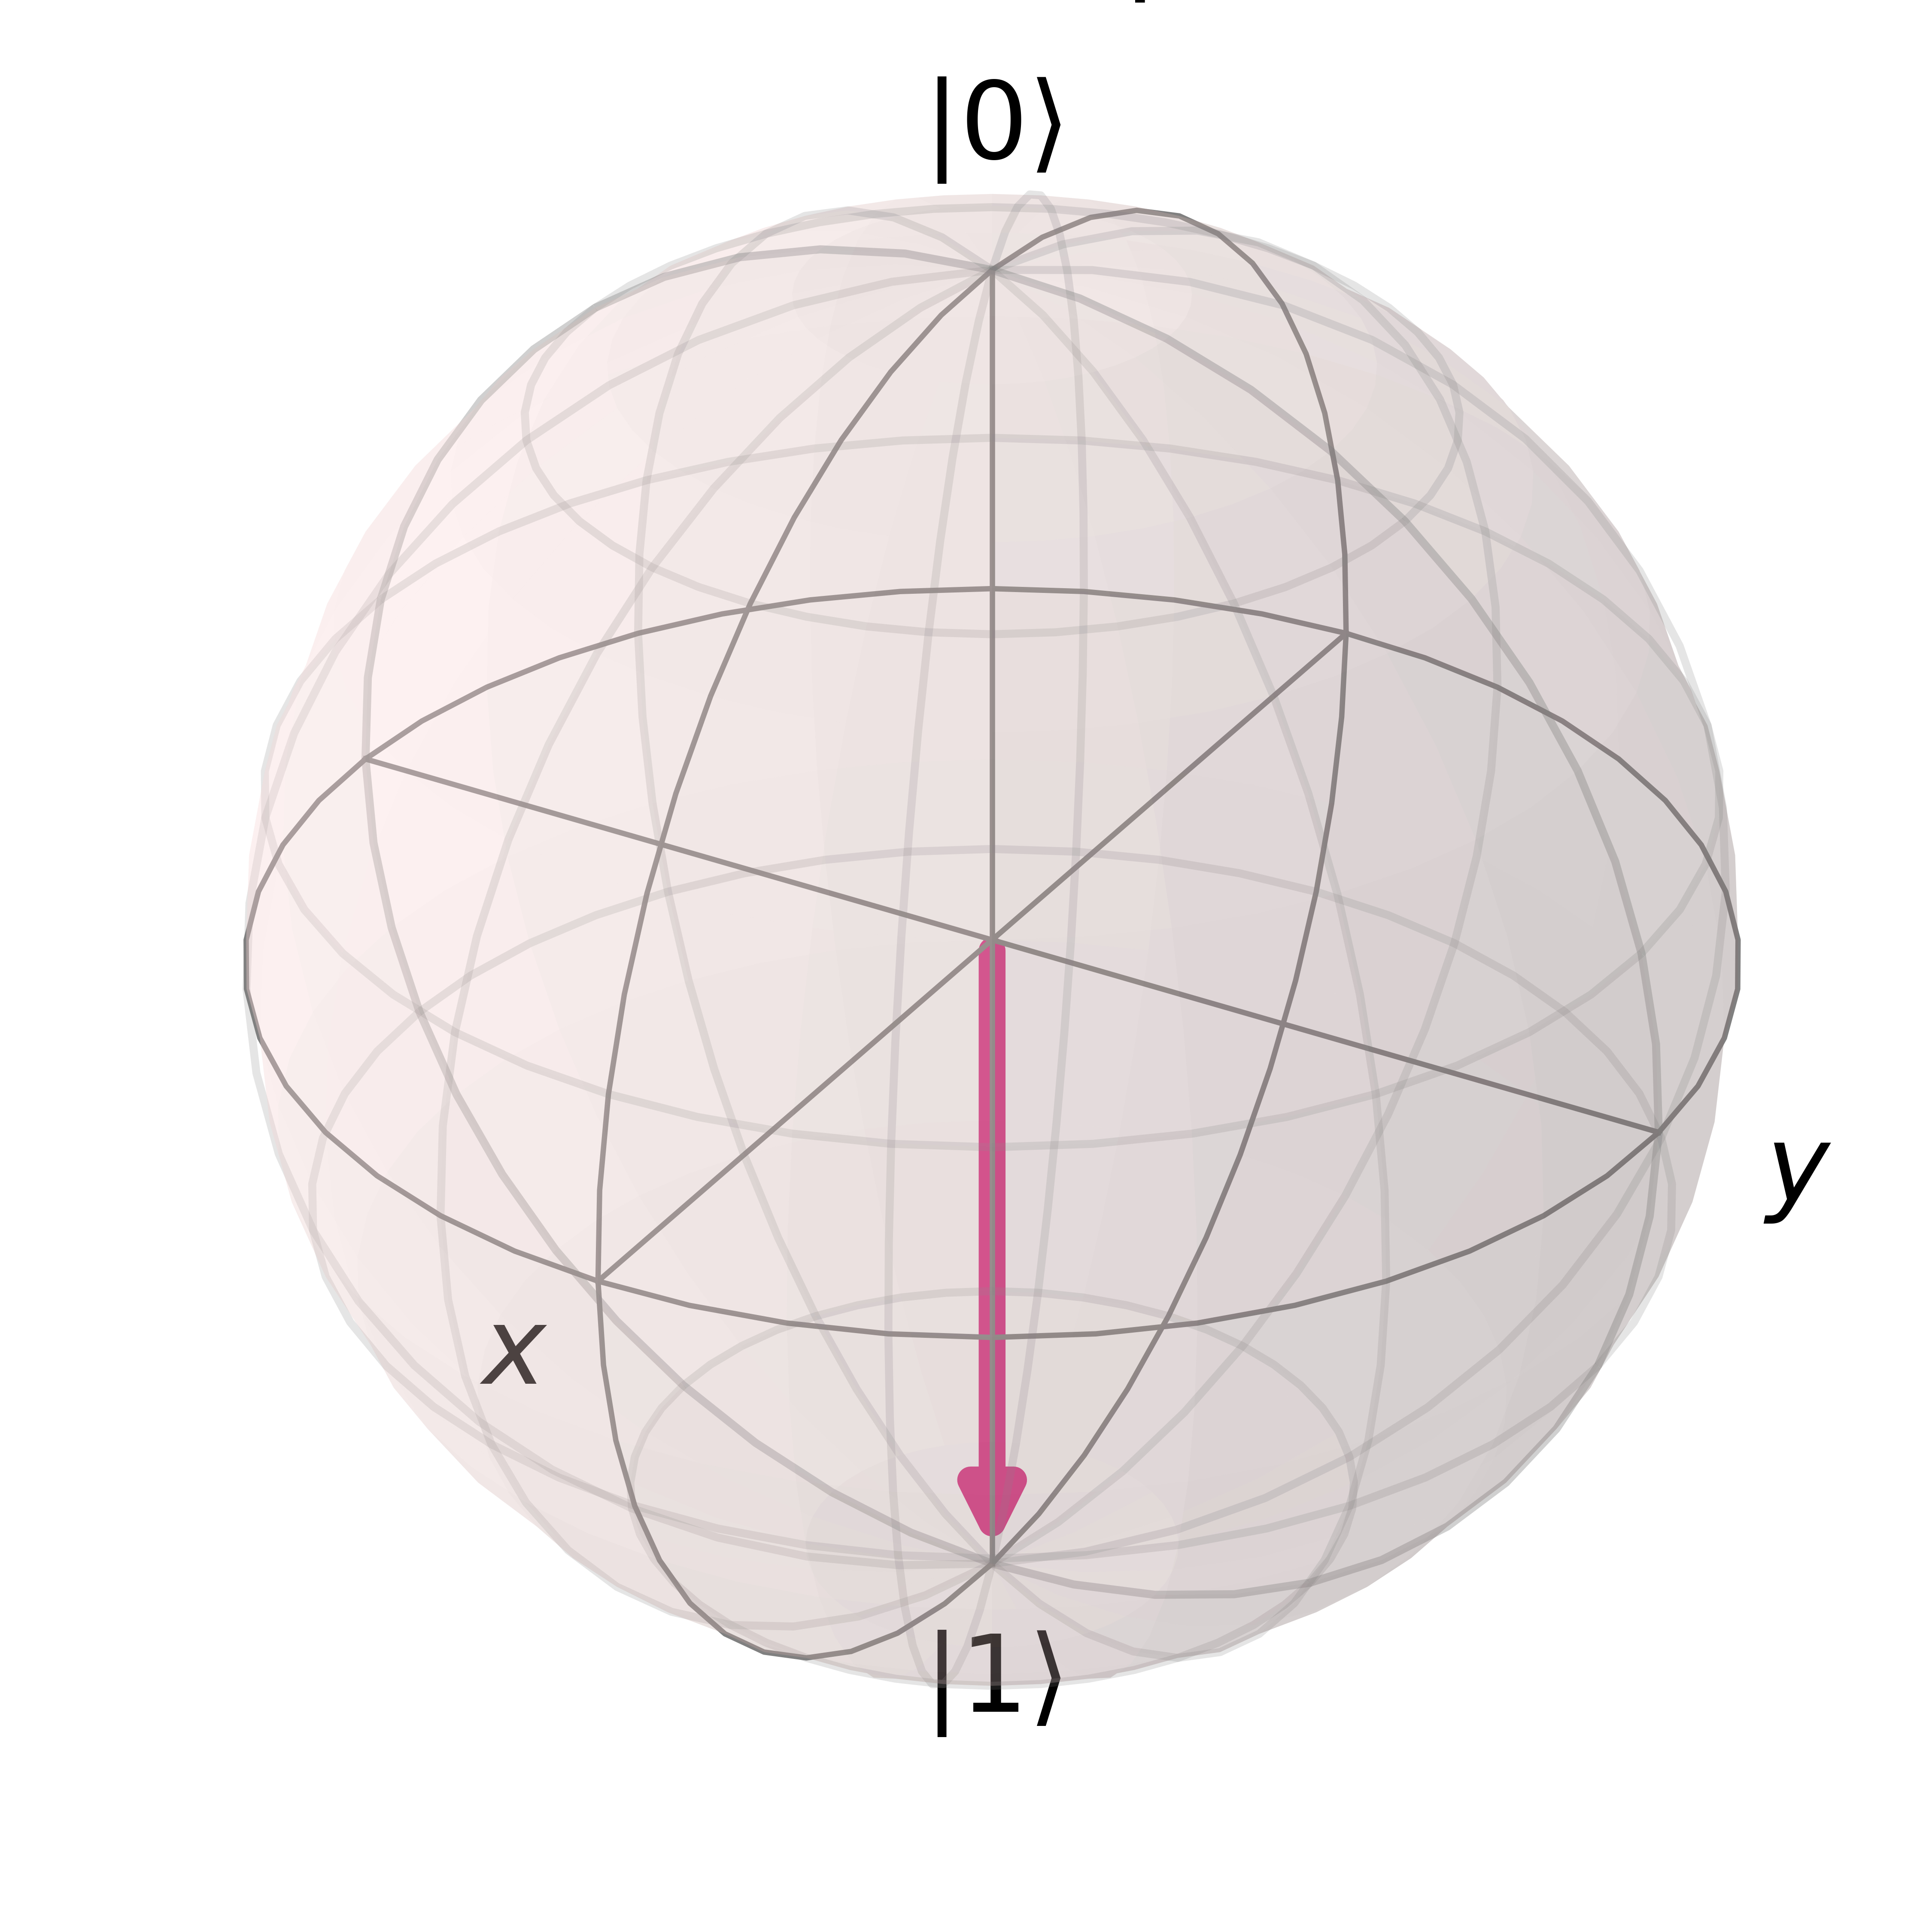
\includegraphics[width=.9\textwidth]{bloch_one.png}
            \column{.5\textwidth}
            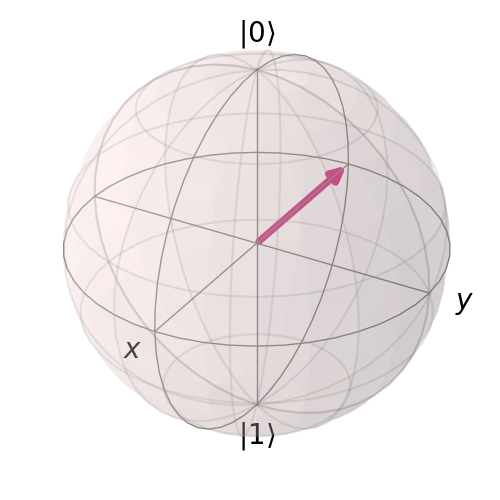
\includegraphics[width=.9\textwidth]{bloch_h_negative.png}
        \end{columns}
    }
\end{frame}

\end{document}
